\documentclass{article}
\usepackage[utf8]{inputenc}
\usepackage[T1]{fontenc}
\usepackage{array}
\usepackage{url}
\usepackage{graphicx}
\usepackage{amsmath,amsfonts}
\usepackage{xspace}
\usepackage{MnSymbol}

\newcommand{\mst}{minimum spanning tree\xspace}

\author{Philip Pickering\\\url{pgpick@gmx.at} \and Thomas Bracht Laumann Jespersen\\\url{ntl316@alumni.ku.dk}}
\title{Advanced Algorithms and Data Structures\\Hand-in 2}
\date{}

\setcounter{MaxMatrixCols}{20}
\begin{document}
\maketitle

%% A couple of tourists wants to visit all monuments in a city. In order to minimize the distance they have to walk, they spend the first day of their holiday implementing a method to find the shortest tour visiting each monument (TSP). They decide to solve the problem using branch-and-bound, so they have to think of a good lower bound.

\subsubsection*{Prove that 1-tree is a lower bound}

Consider the optimal tour $C^*$ in a graph $G$ and a vertex
$u$. Included in the tour are two edges connecting $u$ to the rest of
the graph, $e_1$ and $e_2$. Let $G'$ be the graph formed from $G$ by
removing $u$ and all its incident edges from $G$. Then we can find a
spanning tree $T^{G'}$ from the optimal solution, by removing
$e_1$ and $e_2$ from $C^*$. The following holds:
\begin{equation}
  c(C^*) = c(e_1) + c(e_2) + c(T^{G'}).\label{eq:opt}
\end{equation}
Next consider a \mst $M$ found in $G'$, and the two lowest-cost
edges $e_1'$, $e_2'$ connecting $u$ to $G'$. It is trivial to see
that:
\begin{equation}
  c(e_1') + c(e_2') \leq c(e_1) + c(e_2),\label{eq:es}
\end{equation}
and we can also state that:
\begin{equation}
  c(M) \leq c(T^{G'}),\label{eq:spant}
\end{equation}
since $M$ and $T^{G'}$ are both spanning trees in $G'$.

Combining equations \eqref{eq:es} and \eqref{eq:spant} gives:
\begin{equation}
  c(e_1') + c(e_2') + c(M) \leq c(e_1) + c(e_2) + c(T^{G'}) \stackrel{\eqref{eq:opt}}{=} c(C^*),
\end{equation}
which proves that the 1-tree is indeed a lower bound on the
optimal tour.

\subsubsection*{Zone LP}
%% \begin{quotation}\itshape
%% The tourists get a new idea for a lower bound that might improve the branch-and-bound algorithm. They observe that you can, for each monument, place a circle centered on the monument such that none of the circles overlap. A tour visiting each city has to travel from somewhere on the boundary of each circle, to the center and out to the boundary again.
%% \end{quotation}
Given a graph $G = (V,E)$ with cost/distance function $c : V \times V
\rightarrow \mathbb{R}$, we can write the following linear program to
maximize the radii of non-overlapping circles drawn around each vertex
(the vertices being the origin):
\[
\begin{array}{lrcll}
\textrm{max.:} & \displaystyle\sum_{i=1}^{|V|} r_i  & & & \\
\textrm{s.t.:} &  r_i+r_j                &\leq & c(v_i,v_j), & \forall i,j\in \{1,\dots,|V|\}, v_i, v_j\in V, i \not = j \\
%%& & & & v_i,v_j\in V\\
& r_i &\geq & 0, & \forall i \in \{1,\dots,|V|\}
\end{array}
\]

\subsubsection*{Zone lower bound}

As is described in the exercise a tour visiting each city has to
travel from somewhere on the circumference of each circle, to its
center and back.

Let $r_1^*,\dots,r_2^*$ be the optimal radii found by solving the
liner program presented in the previous section. Then a lower bound on
the optimal TSP solution is given by:
\[
2\sum_{i=0}^{|V|}r_i^*.
\]

Because the circles are non-overlapping, the optimal solution $C^*$ may
have to travel outside the circles, this is indeed a lower bound.

\subsubsection*{ILP formulation of TSP}

To formulate TSP as an \emph{integer linear program} (ILP), we
introduce decision variables for each edge $x_{ij}$, where $i$, $j \in
\{1,\dots,|V|\}$ and $i<j$, and demand that $x_{ij}\in\{0,1\}$, indicating by
zero that the edge is not included in a tour, and one if it is.

\begin{align*}
  \text{min.:} \sum_{i=1}^{n-1}\sum_{j=i+1}^{n} d_{ij}x_{ij}
\end{align*}
\begin{align*}
  \begin{array}{lrcll}
    \text{s.t.:} & \displaystyle\sum_{k=1}^{i-1}x_{ki} + \displaystyle\sum_{k=i+1}^{n} x_{ik} &= &2, & i\in \{1,\dots,|V|\}\\
                 & \displaystyle\sum_{i,j\in Z} x_{ij} &< &|Z|, & \varnothing \subset Z \subset V\\
                 & x_{ij} &\in & \{0,1\}, & i,j \in \{1,\dots,|V|\}
  \end{array}
\end{align*}

The first constraint specifies that for every vertex $i$, exactly two
edges incident to $i$ must be included in the tour.

The second constraint is concerned with subtour elimination, demanding
that for any non-empty $Z\subset V$, the number of edges that are
entirely in $Z$ (both endpoints in $Z$) must be strictly less than
$|Z|$. Say we have five vertices in a subset $Z$. In order to form a
tour amongst themselves, we would need use six edges, which is
disallowed by this constraint.

The third constraint is our \emph{integrality constraint}, demanding
that we either include an edge completely or not at all.

Removing both integrality constraint and subtour constraint. => assignment problem...

\begin{description}
\item[1-tree] description of algorithm
\item[Zones]
\item[ILP Relaxation]
\end{description}

%% \begin{table}[h!]
%%   \begin{tabular}
    
%%   \end{tabular}
%% \end{table}

\begin{table}[h!]
  \centering
  \begin{tabular}{l|c|c|c|c|c|c}
    & \multicolumn{2}{c|}{knollA} & \multicolumn{2}{|c|}{knollB} & \multicolumn{2}{|c}{knollC} \\
    & Training & Test & Training & Test & Training & Test \\
    \hline
    1-tree & 0.01 & 0.03 & 0.40 & 0.49 & 0.01 & 0.03 \\ 
    Zones & -0.242763 & -0.142026 & -1.629922 & -2.061411 & -0.002435 & -0.001425 \\
  \end{tabular}
  \caption{Error percentages and margins for each of the \textsc{knoll} problems}
  \label{tab:ldaknollerror}
\end{table}

\begin{description}
\item[1-tree] How it performed and reasoning
\item[Zones]
\item[ILP Relaxation]
\end{description}

\begin{itemize}
\item table of results 'inf' when no results
\item relaxation of ILP (Thomas)
\item Description of implementation
\item 
\end{itemize}



\newpage
\begin{enumerate}
  \item Prove that the 1-tree is a lower bound. $\checkmark$
  \item Formulate a linear program that maximizes the radii of such
    non-overlapping circles. $\checkmark$
  \item Describe how a lower bound can be computed from these circles. $\checkmark$
  \item Write an integer linear program for TSP. $\checkmark$
  \item Describe how you would relax the integer linear program of TSP to get a lower bound.
  \item Implement each of the three lower bounds described above (1-tree, zones and relaxation) and use them on each of the three problems. For each problem, report the shortest tour and number of nodes visited for each lower bound method. If the program does not terminate within 10 minutes its fine to just write ‘inf’. (There will be a prize for the group that solves the largest problem with the fewest number of nodes evaluated).
  \item For each of the three lower bound methods, give a brief description why you believe it performed the way it did and how it could be improved. 
\end{enumerate}

%% As small example graph can be found in fig.\ref{fig:exg}.

%% \begin{figure}
%%   \centering
%%   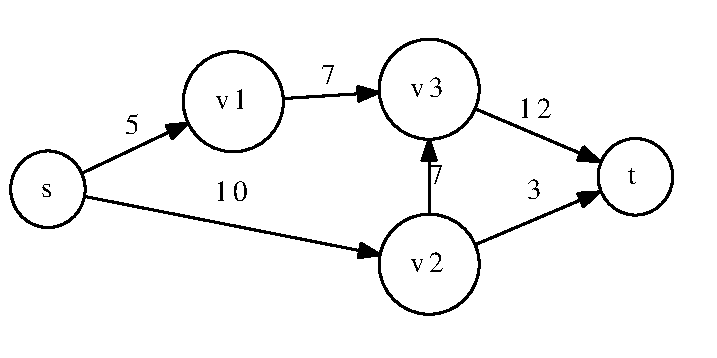
\includegraphics[width=.7\textwidth]{exg.pdf}
%%   \caption{An example max-flow graph}
%%   \label{fig:exg}
%% \end{figure}

%% The linear program corresponding to the graph in fig.~\ref{fig:exg} is
%% the following:
%% \[
%% \begin{array}{lrcll}
%% \textrm{max.:} & f_{s,v_1} + f_{s,v_2} & & &\\
%% \textrm{s.t.:} & f_{s,v_1} &\leq & c(s,v_1) = 5&\\
%%                & f_{s,v_2} &\leq & c(s,v_2) = 10&\\
%%                & f_{v_1,v_3} &\leq & c(v_1,v_3) = 7&\\
%%                & f_{v_2,v_3} &\leq & c(v_1,v_3) = 7&\\
%%                & f_{v_2,t} &\leq & c(v_2,t) = 3&\\
%%                & f_{v_3,t} &\leq & c(v_3,t) = 12&\\
%%                & f_{s,v_1} &= &f_{v_1,v_3}&\\
%%                & f_{s,v_2} &= &f_{v_2,v_3} + f_{v_2,t}&\\
%%                & f_{v_1,v_3} + f_{v_2,v_3} &= &f_{v_3,t}&\\
%% & f_{s,v_1}, f_{s,v_2},f_{v_1,v_3},f_{v_2,v_3},f_{v_2,t}, f_{v_3,t} & \geq & 0\\
%% \end{array}
%% \]

%% We have minimized the above linear program, such that edges with
%% capacity zero have been omitted. Without showing the work of the
%% simplex algorithm, we arrive at the solution: $f_{s,v_1} = 5, f_{s,v_2} =
%% 10$.

%% \section*{\hfill}

%% In order to find the cheapest critical connection we have to identify
%% the \emph{minimal cuts}. Intuitively, if we have a cut $(S, T)$ of our
%% graph and a maximum flow $f$ in that same graph, then the flow from
%% $S$ to $T$ must be equal to capacity across that cut, $c(S,T)$. This
%% means in order to increase the overall flow of the graph, we have to
%% increase the capacities on some of the edges of our minimal cuts.

%% If we only have one such minimal cut, then we simply select the edge
%% with the smallest capacity and increase its capacity. If we have more
%% than one cut, it's not immediately clear which edges to choose.
%% In our example above, we can identify three minimal cuts:
%% \begin{enumerate}
%%   \item $S_1 = \{s\}$, $T_1 = V - \{s\}$
%%   \item $S_2 = \{s,v_2\}$, $T_2 = \{v_1,v_3,t \}$
%%   \item $S_3 = V - \{t\}$, $T_3 = \{t\}$.
%% \end{enumerate}

%% In the first cut we can identify the edge $(s, v_1)$, $c(s,v_1) = 5$,
%% as the cheapest to increase, for $(S_2,T_2)$ the cheapest edge is
%% $(v_2,t)$, $c(v_2,t) = 3$, and this is also the cheapest to increase
%% for $(S_3, T_3)$. If we increase the capacities of these two edges by
%% 1, then we have increased the capacities of all the minimal cuts
%% $(S_i,T_i)$ by 1. In this example the above cuts are still minimal
%% cuts, so the max-flow min-cut theorem tells us that we have increased
%% the maximum flow by 1 (otherwise we should have provoked another
%% minimal cut).

%% Recaptured briefly, in order to find the ``cheapest critical
%% connection'', we need to inspect the minimal cuts and for each of
%% them, select the edge with the smallest capacity to increase. In the
%% end, by the max-flow min-cut property, we will have increased the
%% maximum flow in the entire graph.

%% \section*{\hfill}

%% The dual of the above stated problem can be stated by restating the
%% above program in standard form $Ax\leq b$ along with a coefficent
%% vector $c = \begin{pmatrix} 1 & 1 & 0 & 0 & 0 & 0\end{pmatrix}^T$. The
%%   dual is then given by $A^Ty \geq c$, where we minimize $b^Ty$. $y$
%%   is a vector of size proportional to the number of constraints, in
%%   our case 12, because each of the equality constraints give rise to
%%   two inequalities. Now we can state the dual:

%% \[
%% \begin{array}{cl}
%% \textrm{min.:} & 5y_1 + 10y_2 + 7y_3 + 7y_4 + 3y_5 + 12y_6\\
%% \textrm{s.t.:} &
%%  \begin{bmatrix}%
%%  1 & 0 & 0 & 0 & 0 & 0 & 1 & -1 & 0 & 0 & 0 & 0\\
%%  0 & 1 & 0 & 0 & 0 & 0 & 0 & 0 & 1 & -1 & 0 & 0\\
%%  0 & 0 & 1 & 0 & 0 & 0 & -1 & 1 & 0 & 0 & 1 & -1\\
%%  0 & 0 & 0 & 1 & 0 & 0 & 0 & 0 & -1 & 1 & 1 & -1\\
%%  0 & 0 & 0 & 0 & 1 & 0 & 0 & 0 & -1 & 1 & 0 & 0\\
%%  0 & 0 & 0 & 0 & 0 & 1 & 0 & 0 & 0 & 0 & -1 & 1
%% \end{bmatrix}y
%% \geq
%% \begin{pmatrix}
%%   1\\ 1\\ 0\\ 0\\ 0\\ 0
%% \end{pmatrix}
%% %%\begin{pmatrix} 1\\ 2\end{pmatrix}
%% \end{array}
%% \]
%% A solution to the dual problem is $y_1 = 1, y_2 = 1$ and the rest are
%% zero.

%% \section*{\hfill}

%% In order to model that some of the relay stations aren't owned by
%% the company, we can rephrase the problem as a \emph{minimum-cost flow}
%% problem (29.51), where the cost function:
%% \[
%% a(u,v) = \left\{\begin{array}{ll}1,&\text{if $u$ or $v$ is not owned
%%   by the company}\\ 0,&\text{otherwise.}\end{array}\right.
%% \]
%% Then we can directly apply the definition from the book, because we
%% can require the value of the flow to be exactly $d$.

\end{document}
